\chapter{Architecture}
\label{ARCH}
As discussed in chapter \ref{INTRO}, this thesis aims to explore how the cardinality of DSLs can be used for developing a user-friendly language. The objective of the language is to describe a music-notation and teach novices in programming. Beyond this, the intention is to integrate the DSL in a system which is accessible to everyone. This chapter revises the main idea of the project concept and illustrates the architecture and particular modules. The chapter thereafter elaborates on the implementation of the explained theoretical models.

\section{Idea}
\label{ARCH_IDEA}
To implement the novice-friendly programming language, the already existing project Scalala (cf. section \ref{LIT_PROJ_SCALALA}) was used for the MIDI to music-element mapping (e.g. maps instrument \texttt{Piano} to MIDI channel \texttt{0} (cf. section \ref{THEO_MIDI}). The MIDI approach, was chosen to take advantage of the abstraction to music elements like notes and instruments.

The decision to provide a user-interface as a web-application was made to make the language more accessible and therefore more user friendly. Also, a web application is able to support cross-platform and mobile. As in section \ref{LIT_PROJ} described, all related works offer a desktop application exclusively.

\section{Layered Model}
\label{ARCH_LAYER}
The DSL was implemented as an independent library to decouple the DSL and make it usable for other potential systems. The following figure \ref{IMG_LAYER_ARCH} illustrates the architecture of the application as a whole.

\begin{figure}[h]
\caption{Application Architecture - Layered Model}
\label{IMG_LAYER_ARCH}
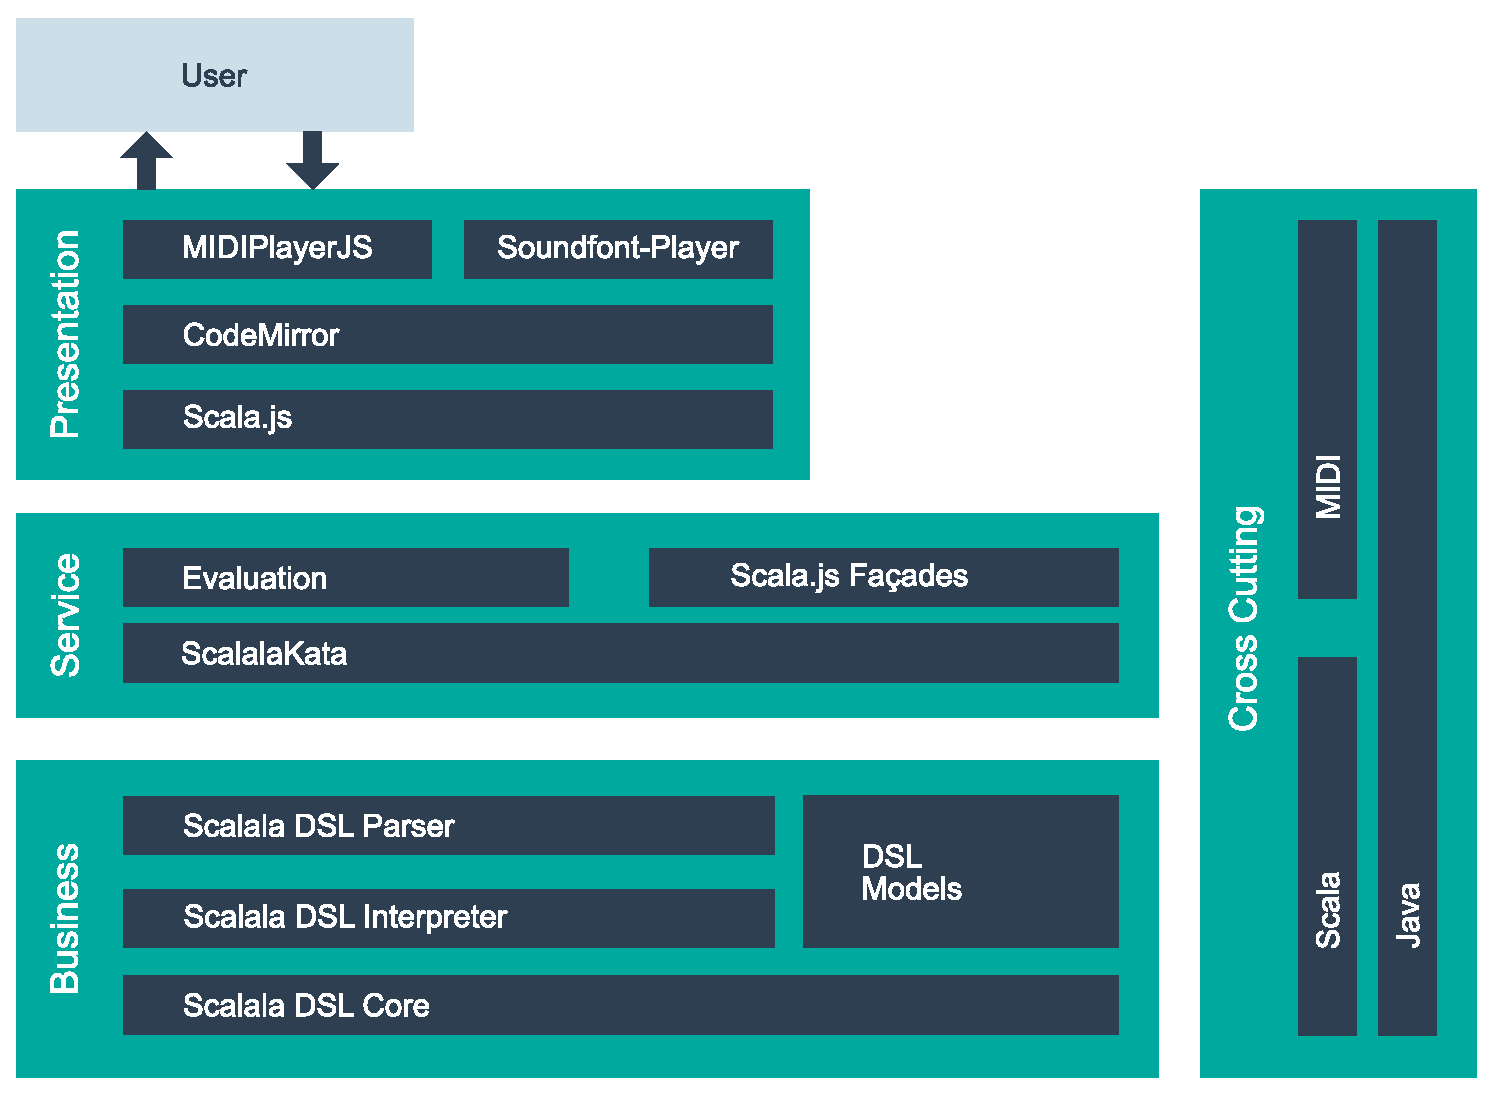
\includegraphics[scale=0.58]{app_layer}
\end{figure}

As seen in the diagram above, the application was implemented in a layered model. Contrary to modern architectures, this application does not follow the microservice-based approach, since the in this thesis implemented system consists of two parts:

\begin{itemize}
\item the web-application en bloc (Service and Presentation Layer) \newline Based on ScalaKata2 (cf. \ref{LIT_PROJ_SCALAKATA2})
\item the DSL library (Business Layer) \newline Based on Scalala (cf. \ref{LIT_PROJ_SCALALA})
\end{itemize}

The layered model was chosen to make use of the simplicity of this architecture and since it is a perfect fit for the classic client server relationship at hand. The DSL library itself was implemented in a model-controller approach (see next section).

The web-application was based on ScalaKata2. According to the advantages of Scala.js, the whole presentation layer was realised through Scala.js. To avoid mixing the Scala.js code base with native JavaScript code, Scala.js façades were written, which would otherwise necessary through the usage of third-party JavaScript libraries. The detailed implementation of the façades is explained in section \ref{IMPL_SCALALAKATA_CSMODEL_CLIENT}. The sound playback through the browser is represented through two libraries: MIDIPlayerJs\footnote{MIDIPlayerJs - \url{https://github.com/grimmdude/MidiPlayerJS}} and Soundfont-Player\footnote{Soundfont-Player - \url{https://github.com/danigb/soundfont-player}}.

Scala as GPL and the MIDI standard was used across all layers (cf. figure \ref{IMG_LAYER_ARCH}). Each layer was implemented in Scala, even the presentation-layer through Scala.js, and the MIDI standard was used to write audio on the DSL side and to read the audio sequences on the front-end side.

\section{DSL Library}
\label{ARCH_DSL}
This section briefly describes the DSL architecture. The DSL follows the \textit{Interpreter} approach. The DSL library reads the DSL script (the input) through the implemented \textit{Reader} at the \textit{Parsing Layer}, which translates the formal input into instructions for the GPL.\cite{Riti2018} The layer acts as the \textit{Lexical Parser} which creates the Abstract Syntax Tree (AST). The AST is used by the interpreter which walks through the AST and translates the results into MIDI. Beyond the theoretical modules, the DSL library, especially the translator relies on a decoupled MIDI class, which is used to create the MIDI result. The results of the MIDI layer could be a hard-disk file, the file encoded as Base64, or other. Besides the specific DSL Layer, each layer uses the already existing Models from Scalala (cf. \ref{THEO_SCALA}). Figure \ref{IMG_DSL_ARCH} illustrates the explained behaviour.

\begin{figure}[h]
\caption{Scalala DSL Architecture}
\label{IMG_DSL_ARCH}
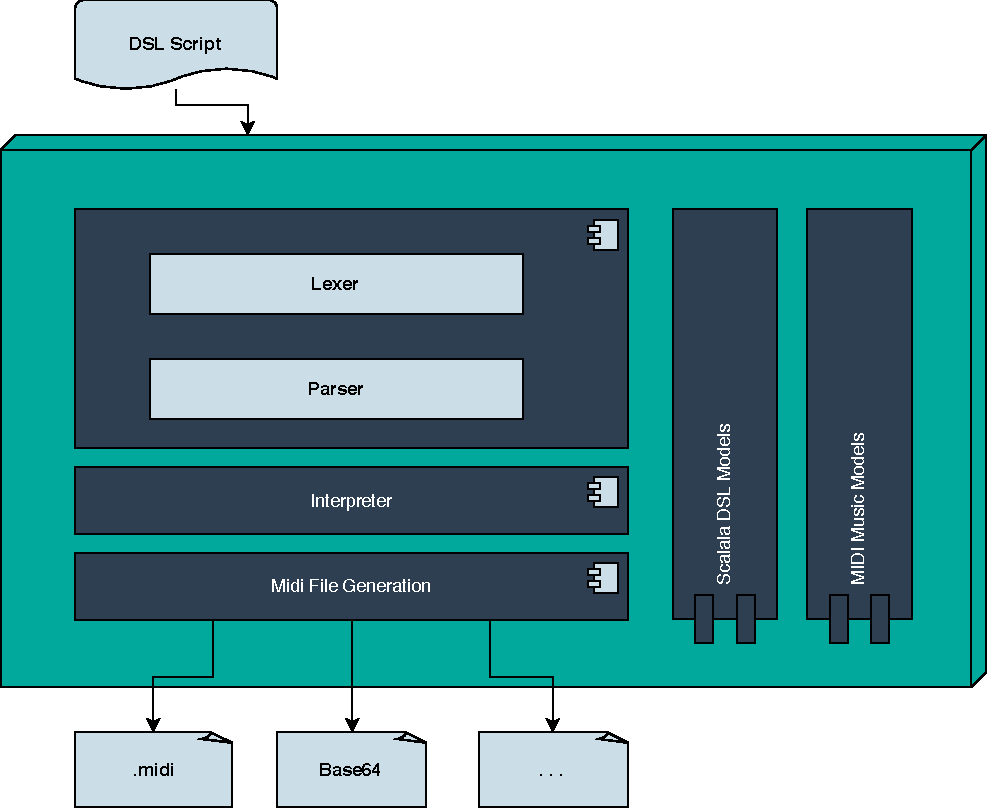
\includegraphics[scale=0.7]{dsl_layer}
\end{figure}

\section{Sequence Model}
\label{ARCH_SEQ}
One outstanding feature of the applications architecture is the usage of the query result, especially the MIDI response. Since MIDI-streams are not possible to playback directly by the browser-engine, an approach to playback these files through JavaScript was necessary. To solve this circumstance, two libraries were included. The MIDIPlayerJs converts input sequences first to the JSON format and provides JavaScript events for each MIDI event. These JavaScript events are caught from the Soundfont-Player library to communicate with the browsers \texttt{AudioContext} and playbacks each MIDI event. Figure \ref{IMG_SEQ_ARCH} shows how a user interacts with the entire system.

\begin{figure}[h]
\caption{ScalalaKata Sequence Diagram}
\label{IMG_SEQ_ARCH}
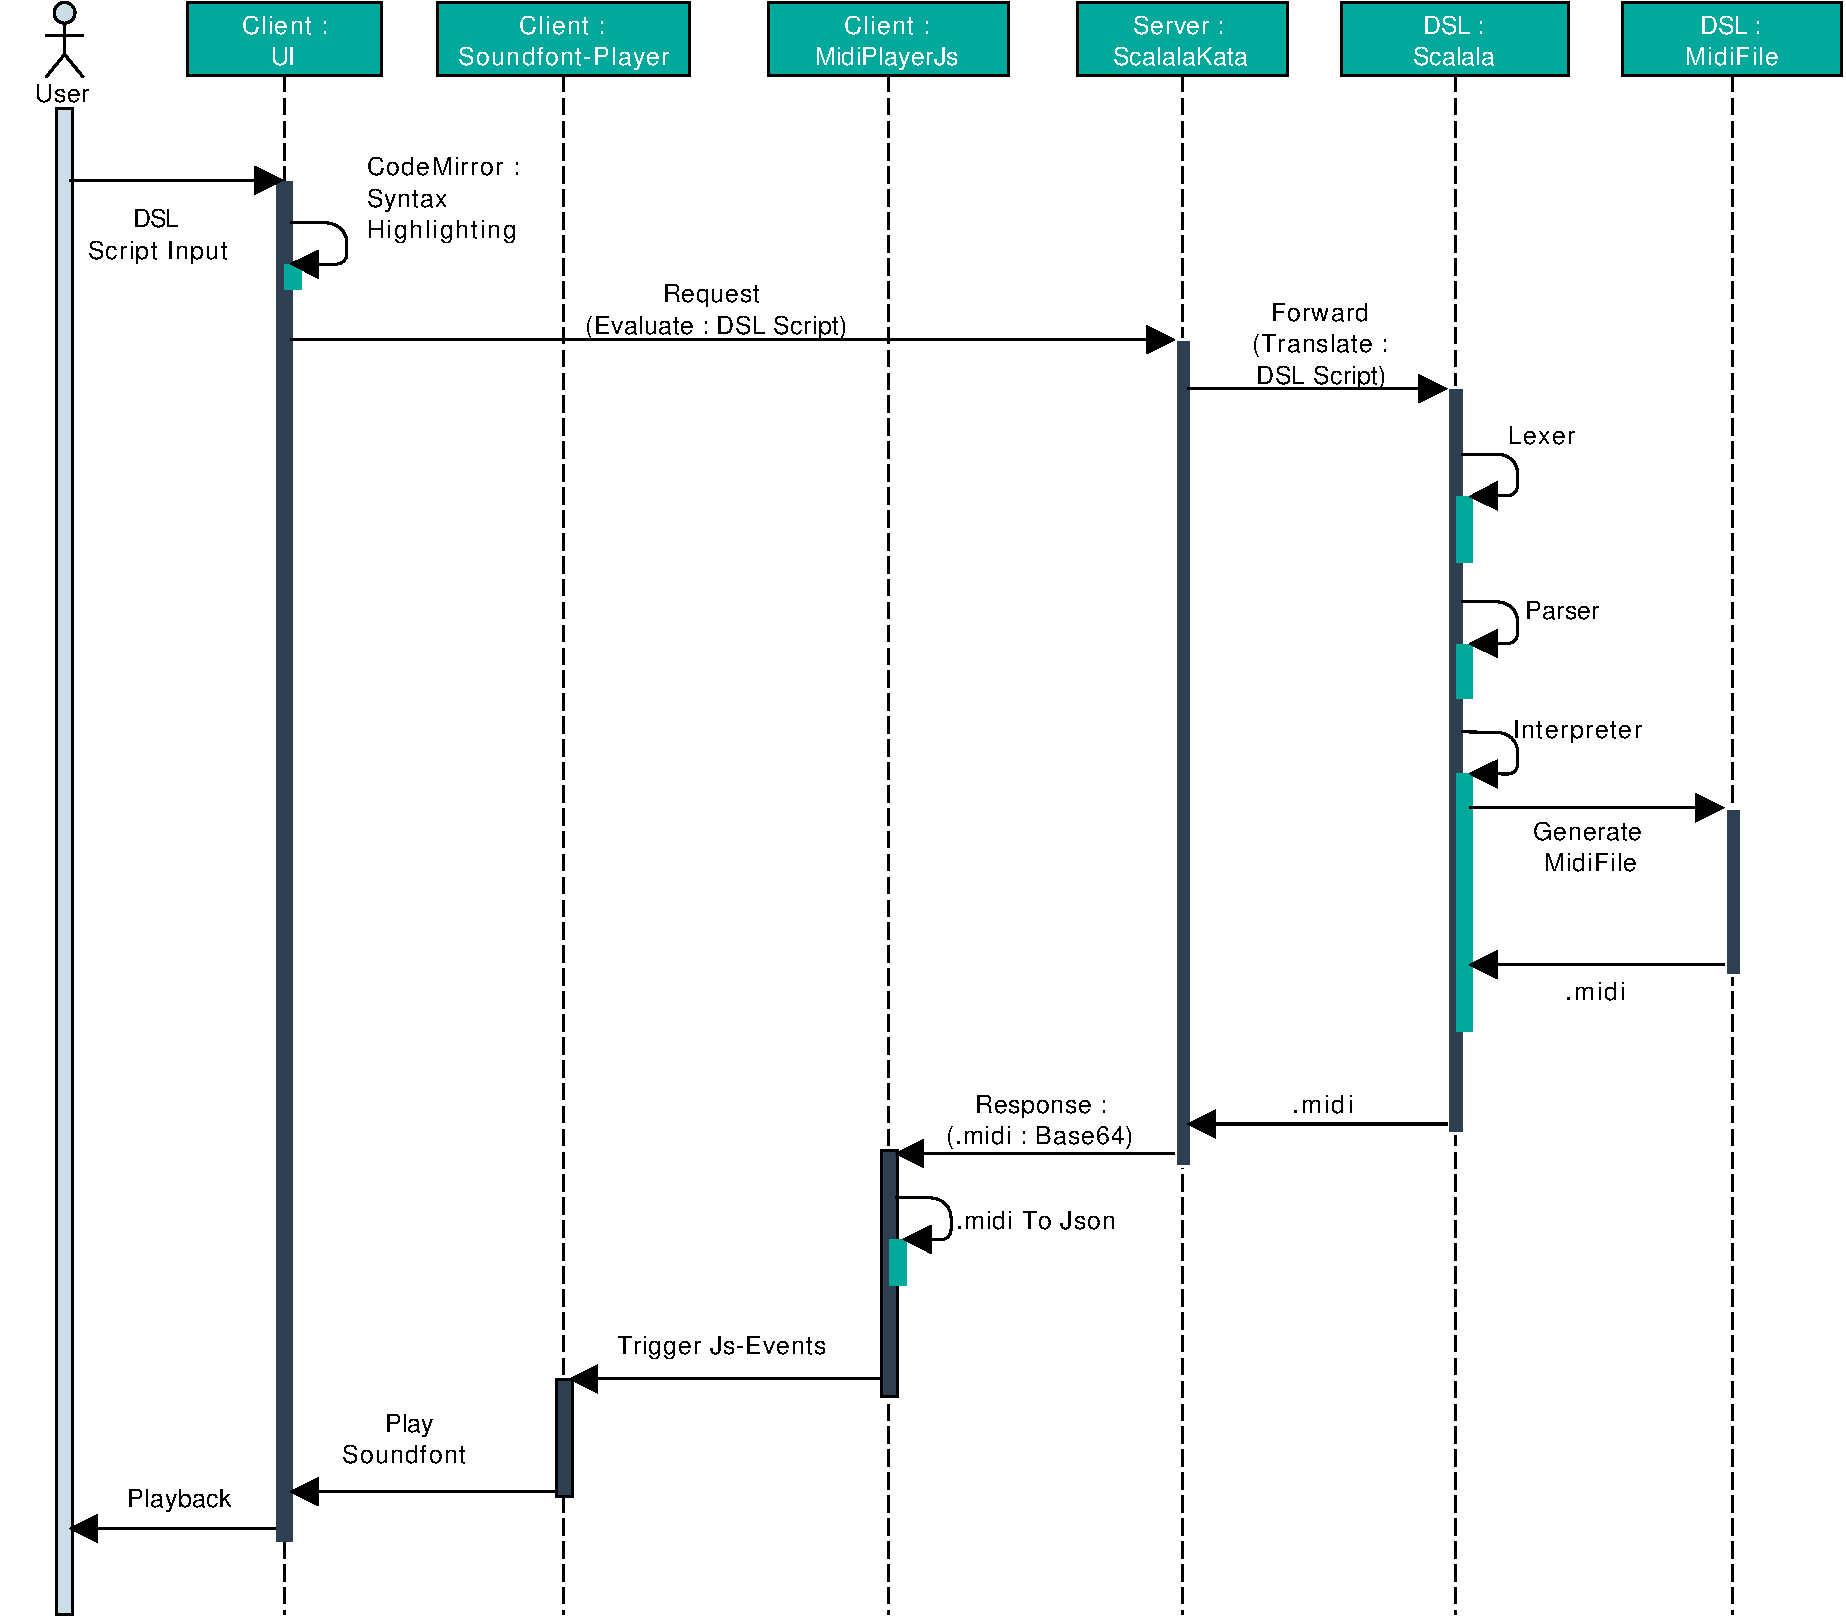
\includegraphics[scale=0.47]{sequence_diagram}
\end{figure}




















